\documentclass{article}

\usepackage{fullpage}
\usepackage{graphicx}
\usepackage{hyperref}
\usepackage{xcolor}

\title{SDSU Git Basics}
\author{SDSU Rocket Project}

\renewcommand{\contentsname}{Contents}

\begin{document}

\maketitle

\begin{center}
	
\includegraphics{rocketlogo.png}
\end{center}

\tableofcontents

\pagebreak

\section{Git Basics}

\subsection{Git Overview}

Git is a Version Control System (VCS) designed to keep track of changes to files across multiple authors and machines.
GitHub is a free public service that hosts the server-side copy (the ``remote'') of all our projects (``repositories'' or ``repos'').
Each user can copy (``clone'') the remote to their machine to have their own copy (their ``local'') that they can edit however they like.
Each repo has a main working tree (usually the ``master'' branch) and can have an infinite number of other ``branches'' that can be edited before their changes are ``merged'' back into master.
Git will automatically check that a merge will not cause conflicts (such as multiple versions of the same file in the same place) and even offers tools to resolve such conflicts.

\subsection{Basic Steps of Git within Rocket Project}

\begin{enumerate}
	\item A branch is created
		\\When created, a branch is identical to the branch it stems from.
	\item Files are created, changed, or deleted
	\item New changes are marked as ``unstaged,'' meaning they are not included for the next commit, and can be made ``staged.''
	\item Those changes are stored as commits
		\\A commit stores the changes in a file since the last commit that includes that file.
		\\Each commit has an associated hash, generated from a SHA1 checksum of the contents of the commit.
		\\Commits are referred to using the first 7 characters of the hash.
		\\Each commit also has at least one line of text, to let you describe what was changed in that commit.
	\item Commits are then uploaded to the remote from your local
		\\This process is called ``pushing'' your commit.
		\\Pushing will upload any commits since your last push, effectively updating the remote to your local.
		\\Always pull before pushing. Someone else could have edited the same files since your last pull, so this helps to prevent conflicts on the remote.
	\item Someone else can then download your commits to their local
		\\This process is called ``pulling'' a commit
		\\Pulling will download any commits since the last pull, effectively updating your local to the remote.
	\item When done, you can ``merge'' your branch into Master via a Pull Request
\end{enumerate}
\subsection{Basic Git Example}

A basic example of the steps to create a branch, write a readme file, and push it to the branch. 
In particular, code examples contain placeholders (formatted in \textit{italics}) that must be replaced manually. \\

\noindent
\texttt{git branch \textit{mybranch}}\verb+          +- Create a new branch named ``mybranch''\\
\texttt{git checkout \textit{mybranch}}\verb+        +- Switch the working directory to the new branch\\
\texttt{vim README.rmd}\verb+                        +- Create and edit \texttt{README.rmd} (vim is a text editor)\\
\texttt{git add README.rmd}\verb+                    +- Stage \texttt{README.rmd} for commit\\
\texttt{git commit -m `Add README.rmd'}\verb+        +- Commit the change with the message `Add README.rmd'\\
\texttt{git pull}\verb+                              +- Fetch any commits, to prevent conflicts when you push\\
\texttt{git push}\verb+                              +- Push your commit to the remote\\

\noindent
While there are commands to create and merge Pull Requests, it's preferred that it is done via GitHub.com.

\pagebreak

\subsection{Basic Commands}

\begin{description}
	\item \texttt{git pull}
		\\``Pull'' retrieves changes from the remote and applies them to the local
		\\\texttt{git pull}
	\item \texttt{git push}
		\\``Push'' sends changes on the local to the remote
		\\\underline{\textbf{ALWAYS PULL BEFORE PUSHING TO AVOID CONFLICTS}}
		\\\texttt{git push}
	\item \texttt{git add}
		\\Stage changes for a commit.
		\\\texttt{git add <filename>}
		\\Don't do \texttt{git add .} because you can accidentally add things you don't want
	\item \texttt{git commit}
		\\Save staged changes into commit
		\\\texttt{git commit [-m <commit message>]}
	\item \texttt{git branch}
		\\List, create, and delete branches.
		\\\texttt{git branch -a} will list all branches (and show an asterisk next to the current branch)
		\\\texttt{git branch <name>} will create a new branch with the specified \texttt{name}
		\\\texttt{git branch -D <name>} will delete the branch with the specified \texttt{name}
	\item \texttt{git checkout}
		\\Switch to a branch.
		\\\texttt{git checkout <branch name>}
	\item \texttt{git cherry-pick}
		\\Apply changes from an existing commit.
		\\\texttt{git cherry-pick <commit hash>}
	\item \texttt{git clone}
		\\Clone a remote repository to the local machine.
		\\\texttt{git clone <url> [target directory]}
	\item \texttt{git diff}
		\\Show the differences between two commits or a commit and the working tree
		\\\texttt{git diff [commit]}
		\\If the \texttt{commit} is not specified, it will compare against the most recent
	\item \texttt{git status}
		\\Show working tree status (staged and unstaged changes, etc...).
		\\\texttt{git status}
	\item \texttt{git log}
		\\Show a log of the working tree. Zack prefers it with these settings:
		\\\texttt{git log --oneline --graph}
	\item \texttt{git reset}
		\\Resets the working tree to the specified state. Two useful ways of invoking:
		\\\texttt{git reset --hard [commit]} will discard any changes since \texttt{commit}
		\\\texttt{git reset <filename>} will unstage a file
		\\If no \texttt{commit} is specified, the most recent will be assumed
\end{description}

\pagebreak

\subsection{Graphical representation}

\begin{center}
	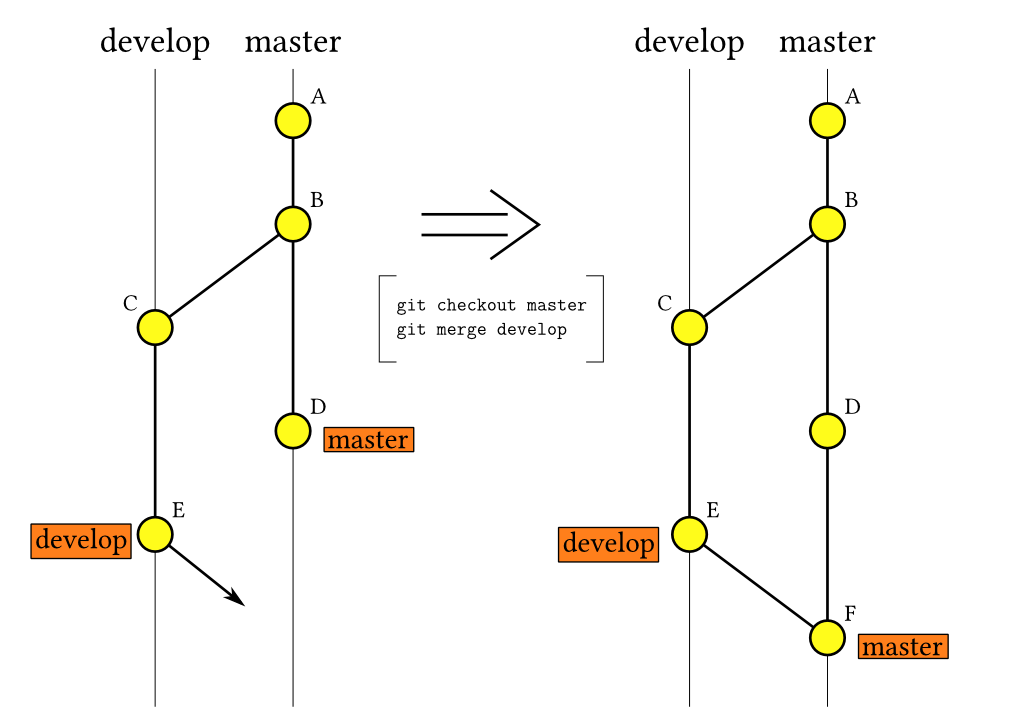
\includegraphics[width=15cm]{commit-merge.png}
\end{center}

Events in the image above:

\begin{enumerate}
	\item Commit A is created and pushed to master
	\item Commit B is created and pushed to master
	\item The branch ``develop'' is created from  master after Commit B
	\item Commit C is created and pushed to develop
	\item Commit D is created and pushed to Master
		\\Note that a commit on one branch does not affect any other branch
	\item Commit E is created and pushed to develop
	\item Develop is merged into Master as Commit F
\end{enumerate}

\

As of point F, all commits on develop are on Master. Master has gained the new features, bugfixes, etc, that were created in develop without having to experience any bugs or errors during the development of commits C and E. This way, only functioning code is on Master.

\pagebreak

\section{Contribution}

\subsection{Contribution Procedure}

\begin{enumerate}
	\item Find an issue on the GitHub page, find something to add, etc.
	\item Create a new branch from Master (or another appropriate branch) to address it
		\\ Your branch should be named appropriately.
		\\ For example, if you are adding documentation for an imaginary BHQQ system, your branch would be named \texttt{bhqq-documentation}
		\\Alternatively, SemVer verion numbers can use used, such as in the FAR-MARS repo.
	\item Commit your changes as you work
		\\You should commit changes as you make them, not everything in one large block. This makes it easier to reference specific changes, especially during review.
		\\Commit messages should be short and descriptive.
	\item File a Pull Request
		\\The Pull Request title should only be a few words, \textit{e.g.} \texttt{Add BHQQ Documentation}.
		\\In the Pull Request message (or in the comments), reference the issue (if any) that you are addressing.
		\\GitHub has an automatic system, where you only need to type the issue number (\textit{e.g.} \texttt{\#10})
	\item Assign reviewers
		\\A pull request into Master can only be accepted if the changes have been approved by at least one other person who has write access to Master.
		\\You should assign someone who is related to the content of your Pull Request (\textit{e.g.} the person who wrote the BHQQ system that you are writing documentation for)
		\\More than one person can be assigned to review your Pull Request.
	\item Make changes
		\\The reviewer may request changes to be made before they approve your Pull Request.
		\\Your Pull Request will also need to be re-approved if you push more commits to your branch before it is merged.
	\item Pull Request Merged
		\\Once all reviewers have approved your Pull Request, it can be merged into Master.
\end{enumerate}

\subsection{Contribution Guidelines}

\begin{itemize}
	\item Create a separate branch for each major change/feature.
		\\This allows us to accept/reject on a feature-by-feature basis.
	
	\item The name of your PR should be short and descriptive.
		\\If you cannot fit everything into a few words, you can expand on additional lines or by further explaining in the PR comments.
	
	\item Your PR \textbf{must} be reviewed by at least one other person.
		\\This person should be someone related to the PR 
		\\(\textit{e.g.} whoever wrote whatever it is that you are modifying).
	\item Commit names should be short, descriptive, and unique.
		\\Pushing six commits in a row all named \texttt{code formatting} helps absolutely no one in understand what is being changed and where.
		\\Additionally, a commit name such as \texttt{Changed README.md} is equally unhelpful. Be sure to include what changes were made.
		If too many changes were made, include the gist of it (e.g. ``Restructure Section 2'') and include a more detailed description in the commit description.
\end{itemize}

\pagebreak

\subsection{How to Improve the Project}

In order to continually improve the project, it is important to take full advantage of the features of GitHub.
This means using features such as Issues, Labels, and Milestones.
These features are completely contained inside the GitHub web interface (or in their graphical client, if you choose to use it).

\subsubsection{Issues}

Anyone can file an issue in the repo. An issue doesn't necessarily need to be an ``issue,'' they are just used to keep track of
any bugs, feature requests, suggested changes, and things of that sort that need to be addressed.
\\

\noindent
All issues, like all Pull Requests, have as associated number and name. For example, the most recent issue filed is titled \texttt{\#9:~Cross Platform Compatibility}. This issue can be referenced anywhere in the repo with just ``\#9'' and GitHub will automatically create a hyperlink to that issue.
\\

\noindent
Issues have three other important fields besides the name and number:
\begin{description}
	\item Assignees
		\\You can assign specific people to work on any issue. It is best to assign the person most likely to resolve the issue. For example, an issue regarding a bug with the way GUI elements are being drawn on the client should be assigned to the person who wrote that section of the client code.
	\item Labels - Described in section~\ref{Labels}
	\item Milestones
		\\You can associate an issue or Pull Request with a specific Milestone, such as ``Convert from Sockets to MQTT'' that would span many issues and Pull Requests, as a way to group them together.
\end{description}

\noindent
It is important that there are always plenty of issues to be resolved.
If you notice a bug, want some new feature, or have an idea for how something could be changed or improved, this is how you let other people know. This is we make progress -- by letting people know what progress needs to be made.

\subsubsection{Labels} \label{Labels}

Labels are markers that can be applied to an issue or a Pull Request in order to help categorize, sort, and filter them.
Multiple labels can be assigned to any issue or Pull Request.
Labels are useful because they allow you to quickly get an idea of what an issue or Pull Request is, and they allow you to filter the list of issues and Pull Requests to only show those with certain labels.
\\

\noindent
New labels can be created or removed at any time. Currently, these exist:
\begin{itemize}
	\item Suggestion
	\item Bug
	\item Documentation
	\item Duplicate
	\item Feature Request
	\item Help Wanted
	\item Question
\end{itemize}

\noindent
If you ever feel that there is no label suitable for your issue or Pull Request, you can always create a new one to fill the hole.

\pagebreak

\section{Documentation}

\subsection{Guidelines}

\begin{itemize}
	\item \textbf{EVERYTHING} must be documented
		\begin{itemize}
			\item All new features
			\item Any new dependencies
			\item \textit{Any} changes that would make current documentation incorrect
		\end{itemize}	
	\item General information (Dependencies, basic operation and descriptions) belong in the repo's README
	\item All code must be thoroughly commented
		\\You will probably not be here in a few years, and it would be best if the next generation can understand how everything works.
\end{itemize}
\end{document}